\documentclass{standalone}
\usepackage{graphicx}	
\usepackage{amssymb, amsmath}
\usepackage{color}

\usepackage{tikz}
\usetikzlibrary{arrows.meta, backgrounds, math}
\usepackage{pgfmath}

\definecolor{light}{RGB}{220, 188, 188}
\definecolor{mid}{RGB}{185, 124, 124}
\definecolor{dark}{RGB}{143, 39, 39}
\definecolor{highlight}{RGB}{180, 31, 180}
\definecolor{light_teal}{RGB}{107, 142, 142}
\definecolor{mid_teal}{RGB}{72, 117, 117}
\definecolor{dark_teal}{RGB}{29, 79, 79}
\definecolor{gray10}{gray}{0.1}
\definecolor{gray20}{gray}{0.2}
\definecolor{gray30}{gray}{0.3}
\definecolor{gray40}{gray}{0.4}
\definecolor{gray60}{gray}{0.6}
\definecolor{gray70}{gray}{0.7}
\definecolor{gray80}{gray}{0.8}
\definecolor{gray90}{gray}{0.9}
\definecolor{gray95}{gray}{0.95}

\tikzmath{
  function warp(\x, \p) {
    if \x > 0 then {
      return +2 * (+\x / 2)^(\p);
    } else {
      return -2 * (-\x / 2)^(\p);
    };
  };
}

\begin{document}

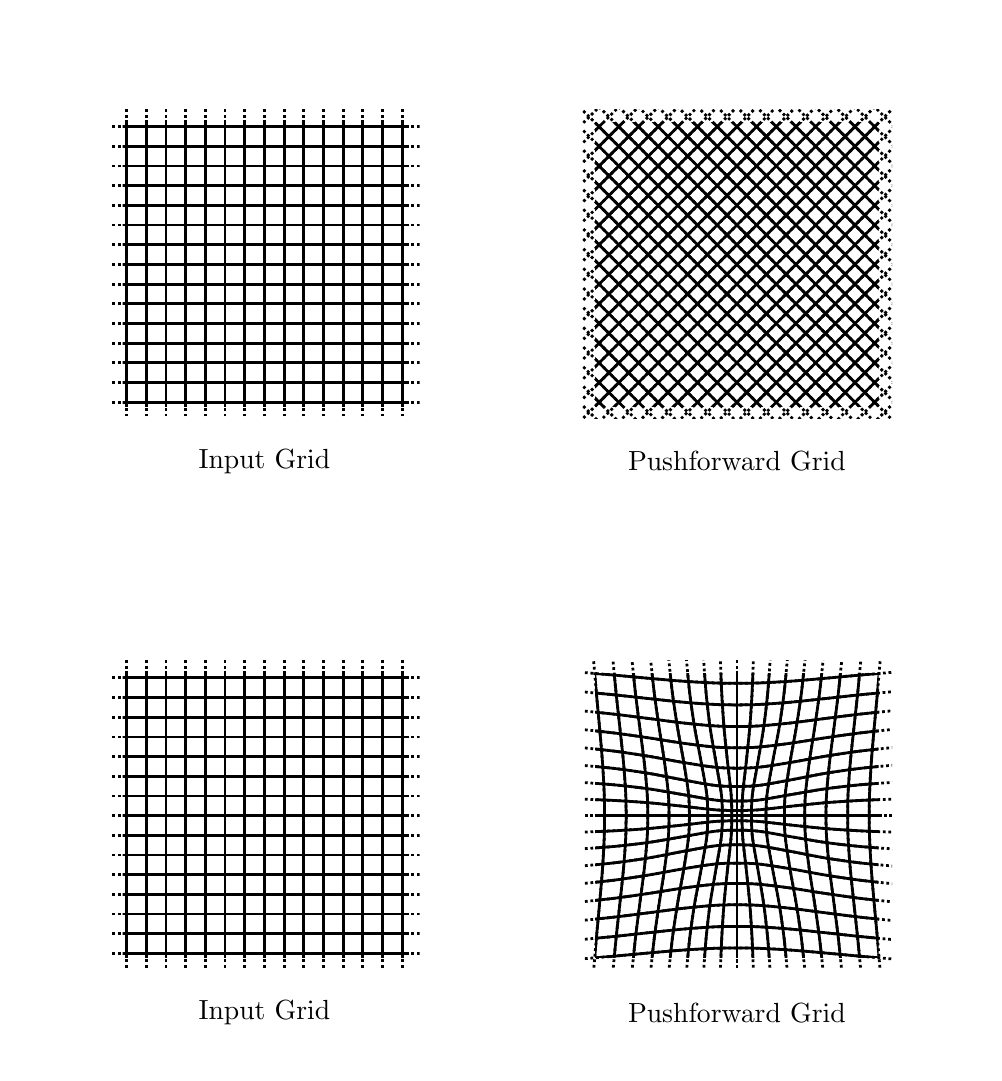
\begin{tikzpicture}[scale=1.0]

  \begin{scope}[shift={(0, 0)}]
    \draw[white] (-3, -3) rectangle (3, 3);
    
    \begin{scope}
      \clip (-1.8, -1.8) rectangle (1.8, 1.8);
      \foreach \y in { -2, -1.75, ..., 2.1 } {
        \draw[black, line width=1] (-2, \y) -- (2, \y);
      }
      \foreach \x in { -2, -1.75, ..., 2.1 } {
        \draw[black, line width=1] (\x, -2) -- (\x, 2);
      }
    \end{scope}
    
    \begin{scope}
      \clip (-1.96, -1.96) rectangle (1.97, 1.97);
      \foreach \y in { -2, -1.75, ..., 2.1 } {
        \draw[black, densely dotted, line width=1] (-2, \y) -- (2, \y);
      }
      \foreach \x in { -2, -1.75, ..., 2.1 } {
        \draw[black, densely dotted, line width=1] (\x, -2) -- (\x, 2);
      }
    \end{scope}
    \node at (0, -2.5) { Input Grid };
  \end{scope}

  \begin{scope}[shift={(6, 0)}]
    \draw[white] (-3, -3) rectangle (3, 3);
    
    \begin{scope}
      \clip (-1.8, -1.8) rectangle (1.8, 1.8);
      \foreach \c in { -5, -4.75, ..., 5.1 } {
        \draw[domain={-2:2}, smooth, samples=10, line width=1, variable=\x] 
          plot (\x, \c - \x);
      }
      \foreach \c in { -5, -4.75, ..., 5.1 } {
        \draw[domain={-2:2}, smooth, samples=10, line width=1, variable=\x] 
          plot (\x, \c + \x);
      }
    \end{scope}
    
    \begin{scope}
      \clip (-1.96, -1.96) rectangle (1.97, 1.97);
      \foreach \c in { -5, -4.75, ..., 5.1 } {
        \draw[domain={-2:2}, smooth, samples=10, line width=1, variable=\x, densely dotted] 
          plot (\x, \c - \x);
      }
      \foreach \c in { -5, -4.75, ..., 5.1 } {
        \draw[domain={-2:2}, smooth, samples=10, line width=1, variable=\x, densely dotted] 
          plot (\x, \c + \x);
      }
    \end{scope}
    \node at (0, -2.5) { Pushforward Grid };
  \end{scope}
  
  \begin{scope}[shift={(0, -7)}]
    \draw[white] (-3, -3) rectangle (3, 3);
    
    \begin{scope}
      \clip (-1.8, -1.8) rectangle (1.8, 1.8);
      \foreach \y in { -2, -1.75, ..., 2.1 } {
        \draw[black, line width=1] (-2, \y) -- (2, \y);
      }
      \foreach \x in { -2, -1.75, ..., 2.1 } {
        \draw[black, line width=1] (\x, -2) -- (\x, 2);
      }
    \end{scope}
    
    \begin{scope}
      \clip (-1.96, -1.96) rectangle (1.97, 1.97);
      \foreach \y in { -2, -1.75, ..., 2.1 } {
        \draw[black, densely dotted, line width=1] (-2, \y) -- (2, \y);
      }
      \foreach \x in { -2, -1.75, ..., 2.1 } {
        \draw[black, densely dotted, line width=1] (\x, -2) -- (\x, 2);
      }
    \end{scope}
    \node at (0, -2.5) { Input Grid };
  \end{scope}
  
  \begin{scope}[shift={(6, -7)}]
    \draw[white] (-3, -3) rectangle (3, 3);
    
    \begin{scope}
      \clip (-1.8, -1.8) rectangle (1.8, 1.8);
      \foreach \y in { -2, -1.75, ..., 2.1 } {
        \draw[domain={-2:2}, smooth, samples=10, line width=1, variable=\x] 
          plot (\x, {\y * (1 - 8 / (10 * (\x * \x + \y * \y) + 10)))});
      }
      \foreach \x in { -2, -1.75, ..., 2.1 } {
        \draw[domain={-2:2}, smooth, samples=10, line width=1, variable=\y] 
          plot ({\x * (1 - 8 / (10 * (\x * \x + \y * \y) + 10))}, \y);
      }
    \end{scope}
    
    \begin{scope}
      \clip (-1.96, -1.96) rectangle (1.97, 1.97);
      \foreach \y in { -2, -1.75, ..., 2.1 } {
        \draw[domain={-2:2}, smooth, samples=10, line width=1, densely dotted, variable=\x] 
          plot (\x, {\y * (1 - 8 / (10 * (\x * \x + \y * \y) + 10)))});
      }
      \foreach \x in { -2, -1.75, ..., 2.1 } {
        \draw[domain={-2:2}, smooth, samples=10, line width=1, densely dotted, variable=\y] 
          plot ({\x * (1 - 8 / (10 * (\x * \x + \y * \y) + 10))}, \y);
      }
    \end{scope}
    \node at (0, -2.5) { Pushforward Grid };
  \end{scope}
    
\end{tikzpicture}

\end{document}  